\newpage
\section{Delimitación de expresiones matemáticas}
\label{sec:del_exp}
Debido a la elección de un modelo sequence to sequence para resolver el problema de reconocimiento y traducción de las expresiones, los símbolos y tipo de expresiones matemáticas a reconocer están limitadas por el conjunto de entrenamiento a utilizar. El presente Trabajo Terminal, se enfocará en reconocer expresiones matemáticas escritas a mano.

La Competición en el Reconocimiento de Expresiones Matemáticas Escritas a Mano \textit{CROHME} de sus siglas en inglés, provee de un conjunto de entrenamiento que consta de casi 10,000 imágenes seperadas en conjuntos de entrenamiento, validación y prueba. Este conjunto de entrenamiento, será el principal conjunto utilizado por el presente Trabajo Terminal.

Existe otro conjunto sobre expresiones matemáticas, fue publicado por \cite{harvard}, se compone cerca de 100,000 imágenes de expresiones matemáticas renderizadas a computadora. Este conjunto solo será utilizado para comprobar como distintos conjuntos de entrenamiento pueden afectar el desempeño del modelo, pues las expresiones renderizadas por computadora, son sustancialmente diferentes de las provistas por CROHME.

Al utilizar el conjunto de entrenamiento CROHME \cite{CROHME} se tomó un análisis de símbolos existentes en dicho conjunto de entrenamiento realizado con ayuda de la herramienta \textbf{CROHME Data Extractor} \cite{EXTRACTOR}. El conteo de apariciones de símbolos arroja las siguientes gráficas de frecuencias clasificando los tipos de símbolos.\\

La primer gráfica muestra la frecuencia de los dígitos del sistema arábigo, donde podemos ver que el dígito \textbf{1} aparece nueve mil cuatrocientos sesenta veces siendo este el de mayor aparición en esta categoría, mientras que el 7 aparece mil veinticinco veces.
\begin{figure}[H]
	\centering
	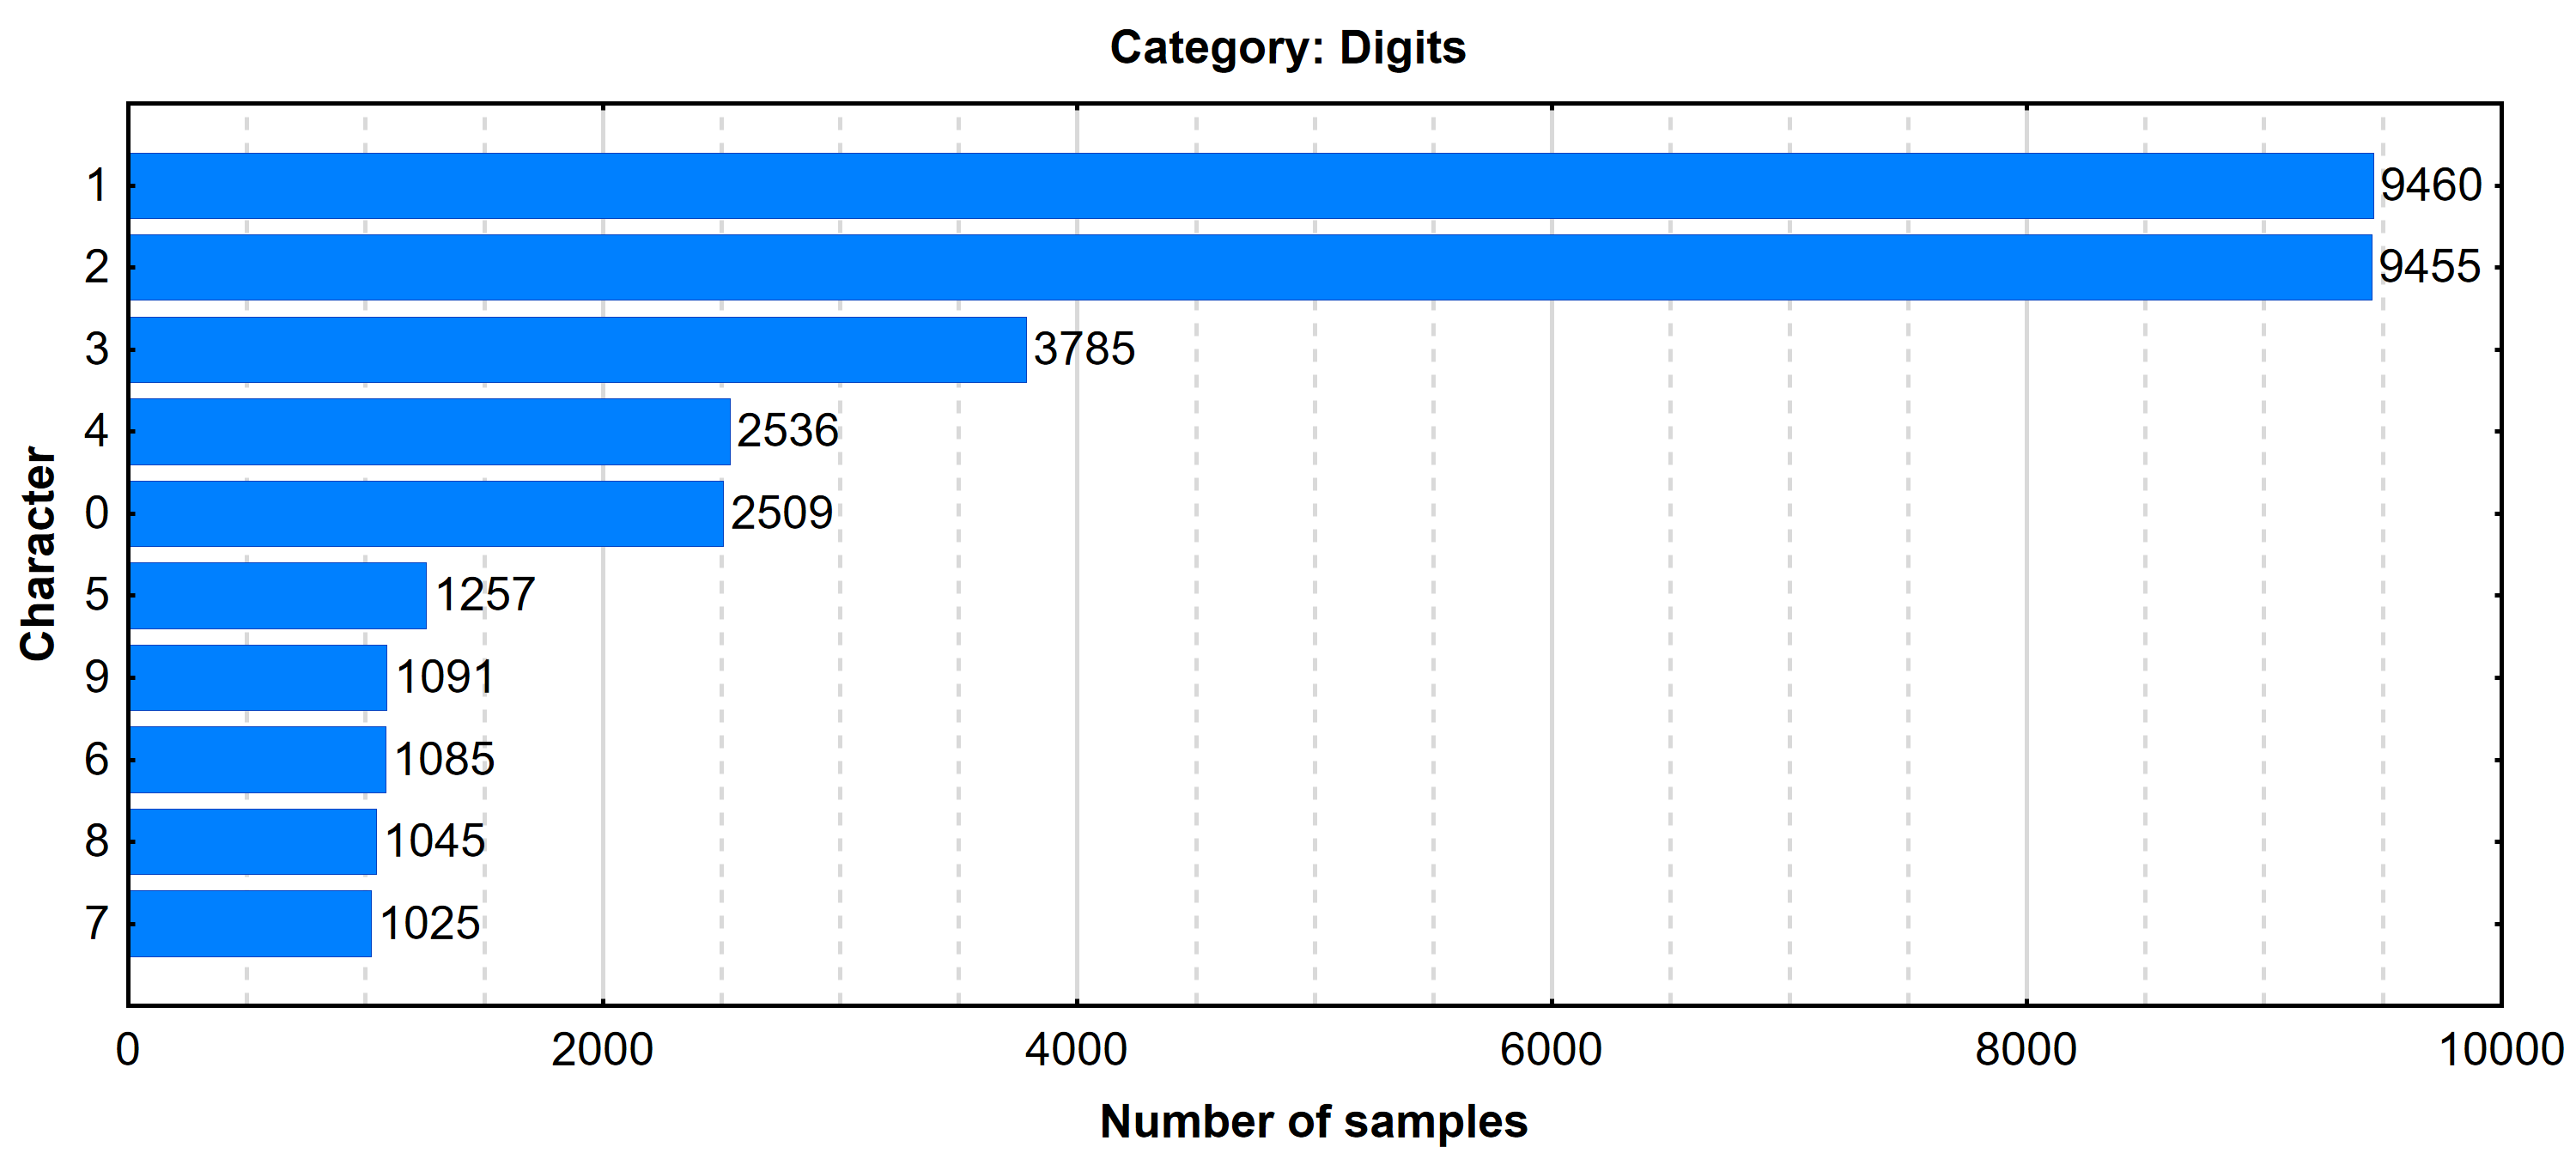
\includegraphics[width=1\textwidth]{capitulo3/imgs/digits_distribution.png}
	\caption{Frecuencia de aparición de dígitos del sistema de numeración arábigo \cite{EXTRACTOR}}
	\label{fig:DigDist}
\end{figure}
\newpage
En el caso de los símbolos matemáticos el de mayor aparición es el símbolo \textbf{-} con doce mil trecientas veintiocho veces. En esta gráfica podemos observar la aparición de símbolos que soportan expresiones que involucren divisiones o funciones trigonométricas o comparadores, incluso cuantificador de existencia aunque con una muy baja frecuencia de tan solo once apariciones.
\begin{figure}[H]
	\centering
	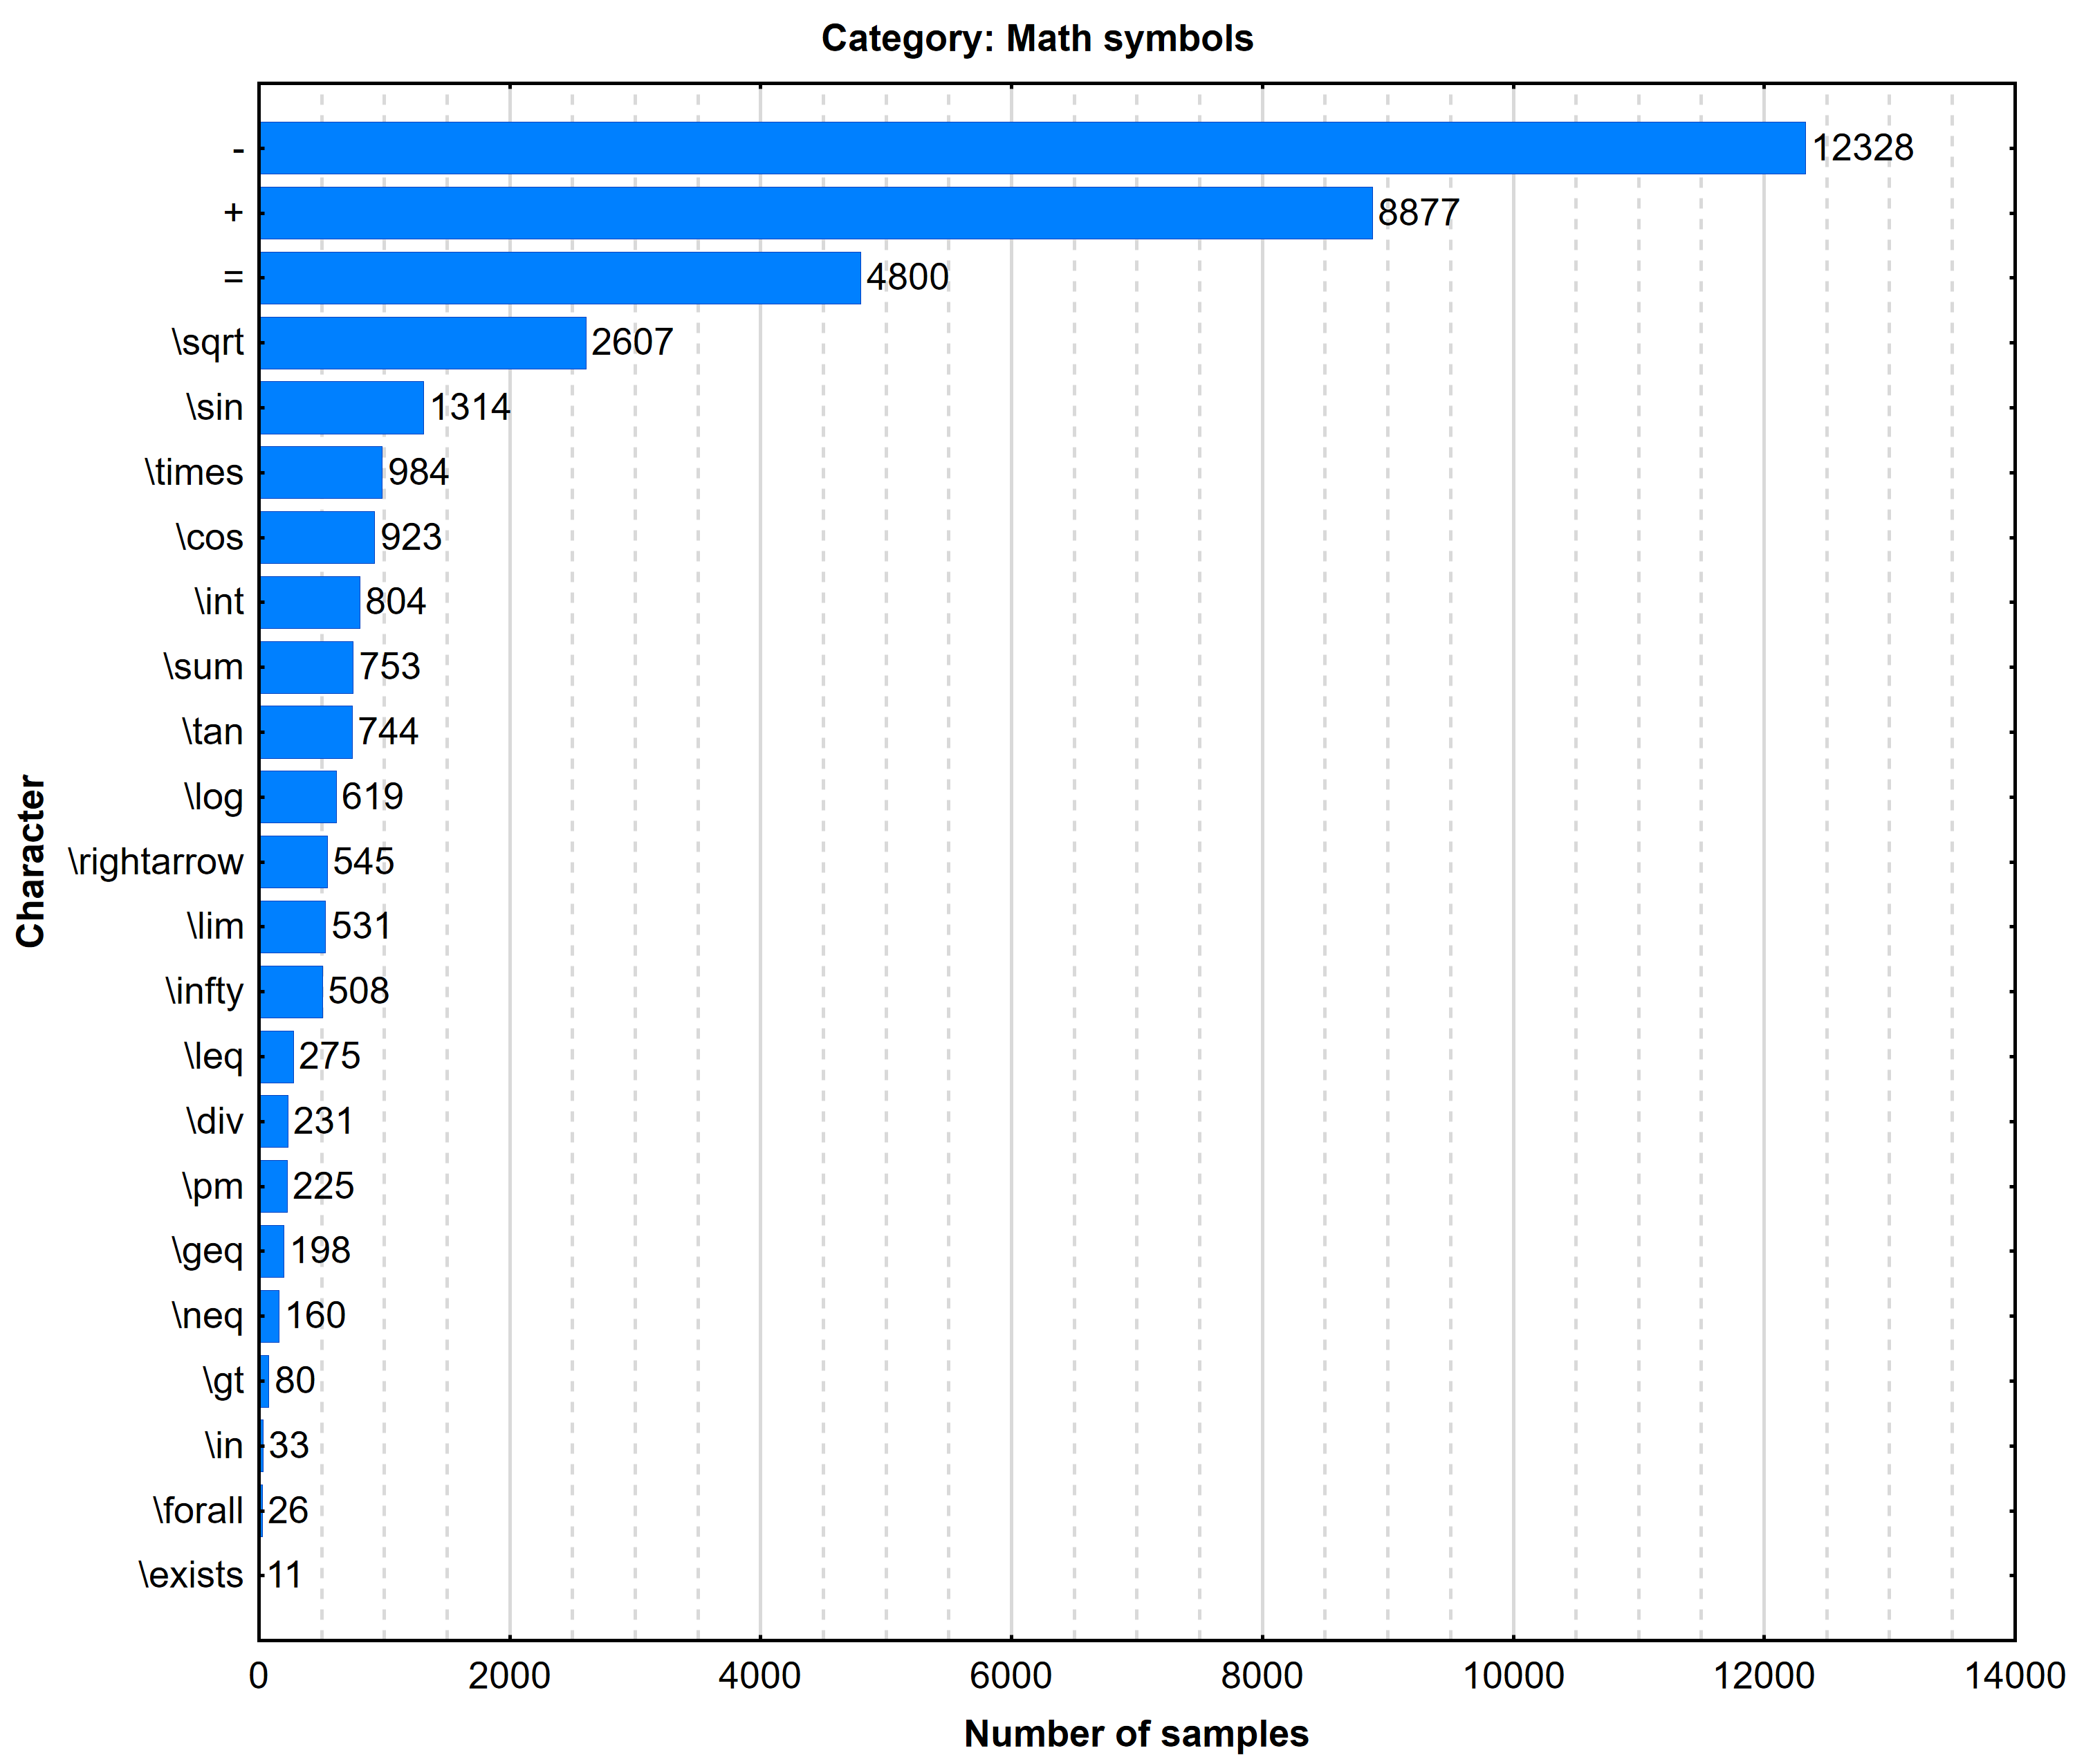
\includegraphics[width=1\textwidth]{capitulo3/imgs/math_symbols_distribution.png}
	\caption{Frecuencia de aparición de símbolos matemáticos \cite{EXTRACTOR}}
	\label{fig:MathSymbols}
\end{figure}
\newpage

En el caso de letras mayúsculas se logró identificar una frecuencia de cuatrocientos sesenta y nueve para el caso de la letra \textbf{C} mientras que para la letra \textbf{I} de noventa y seis.
\begin{figure}[H]
	\centering
	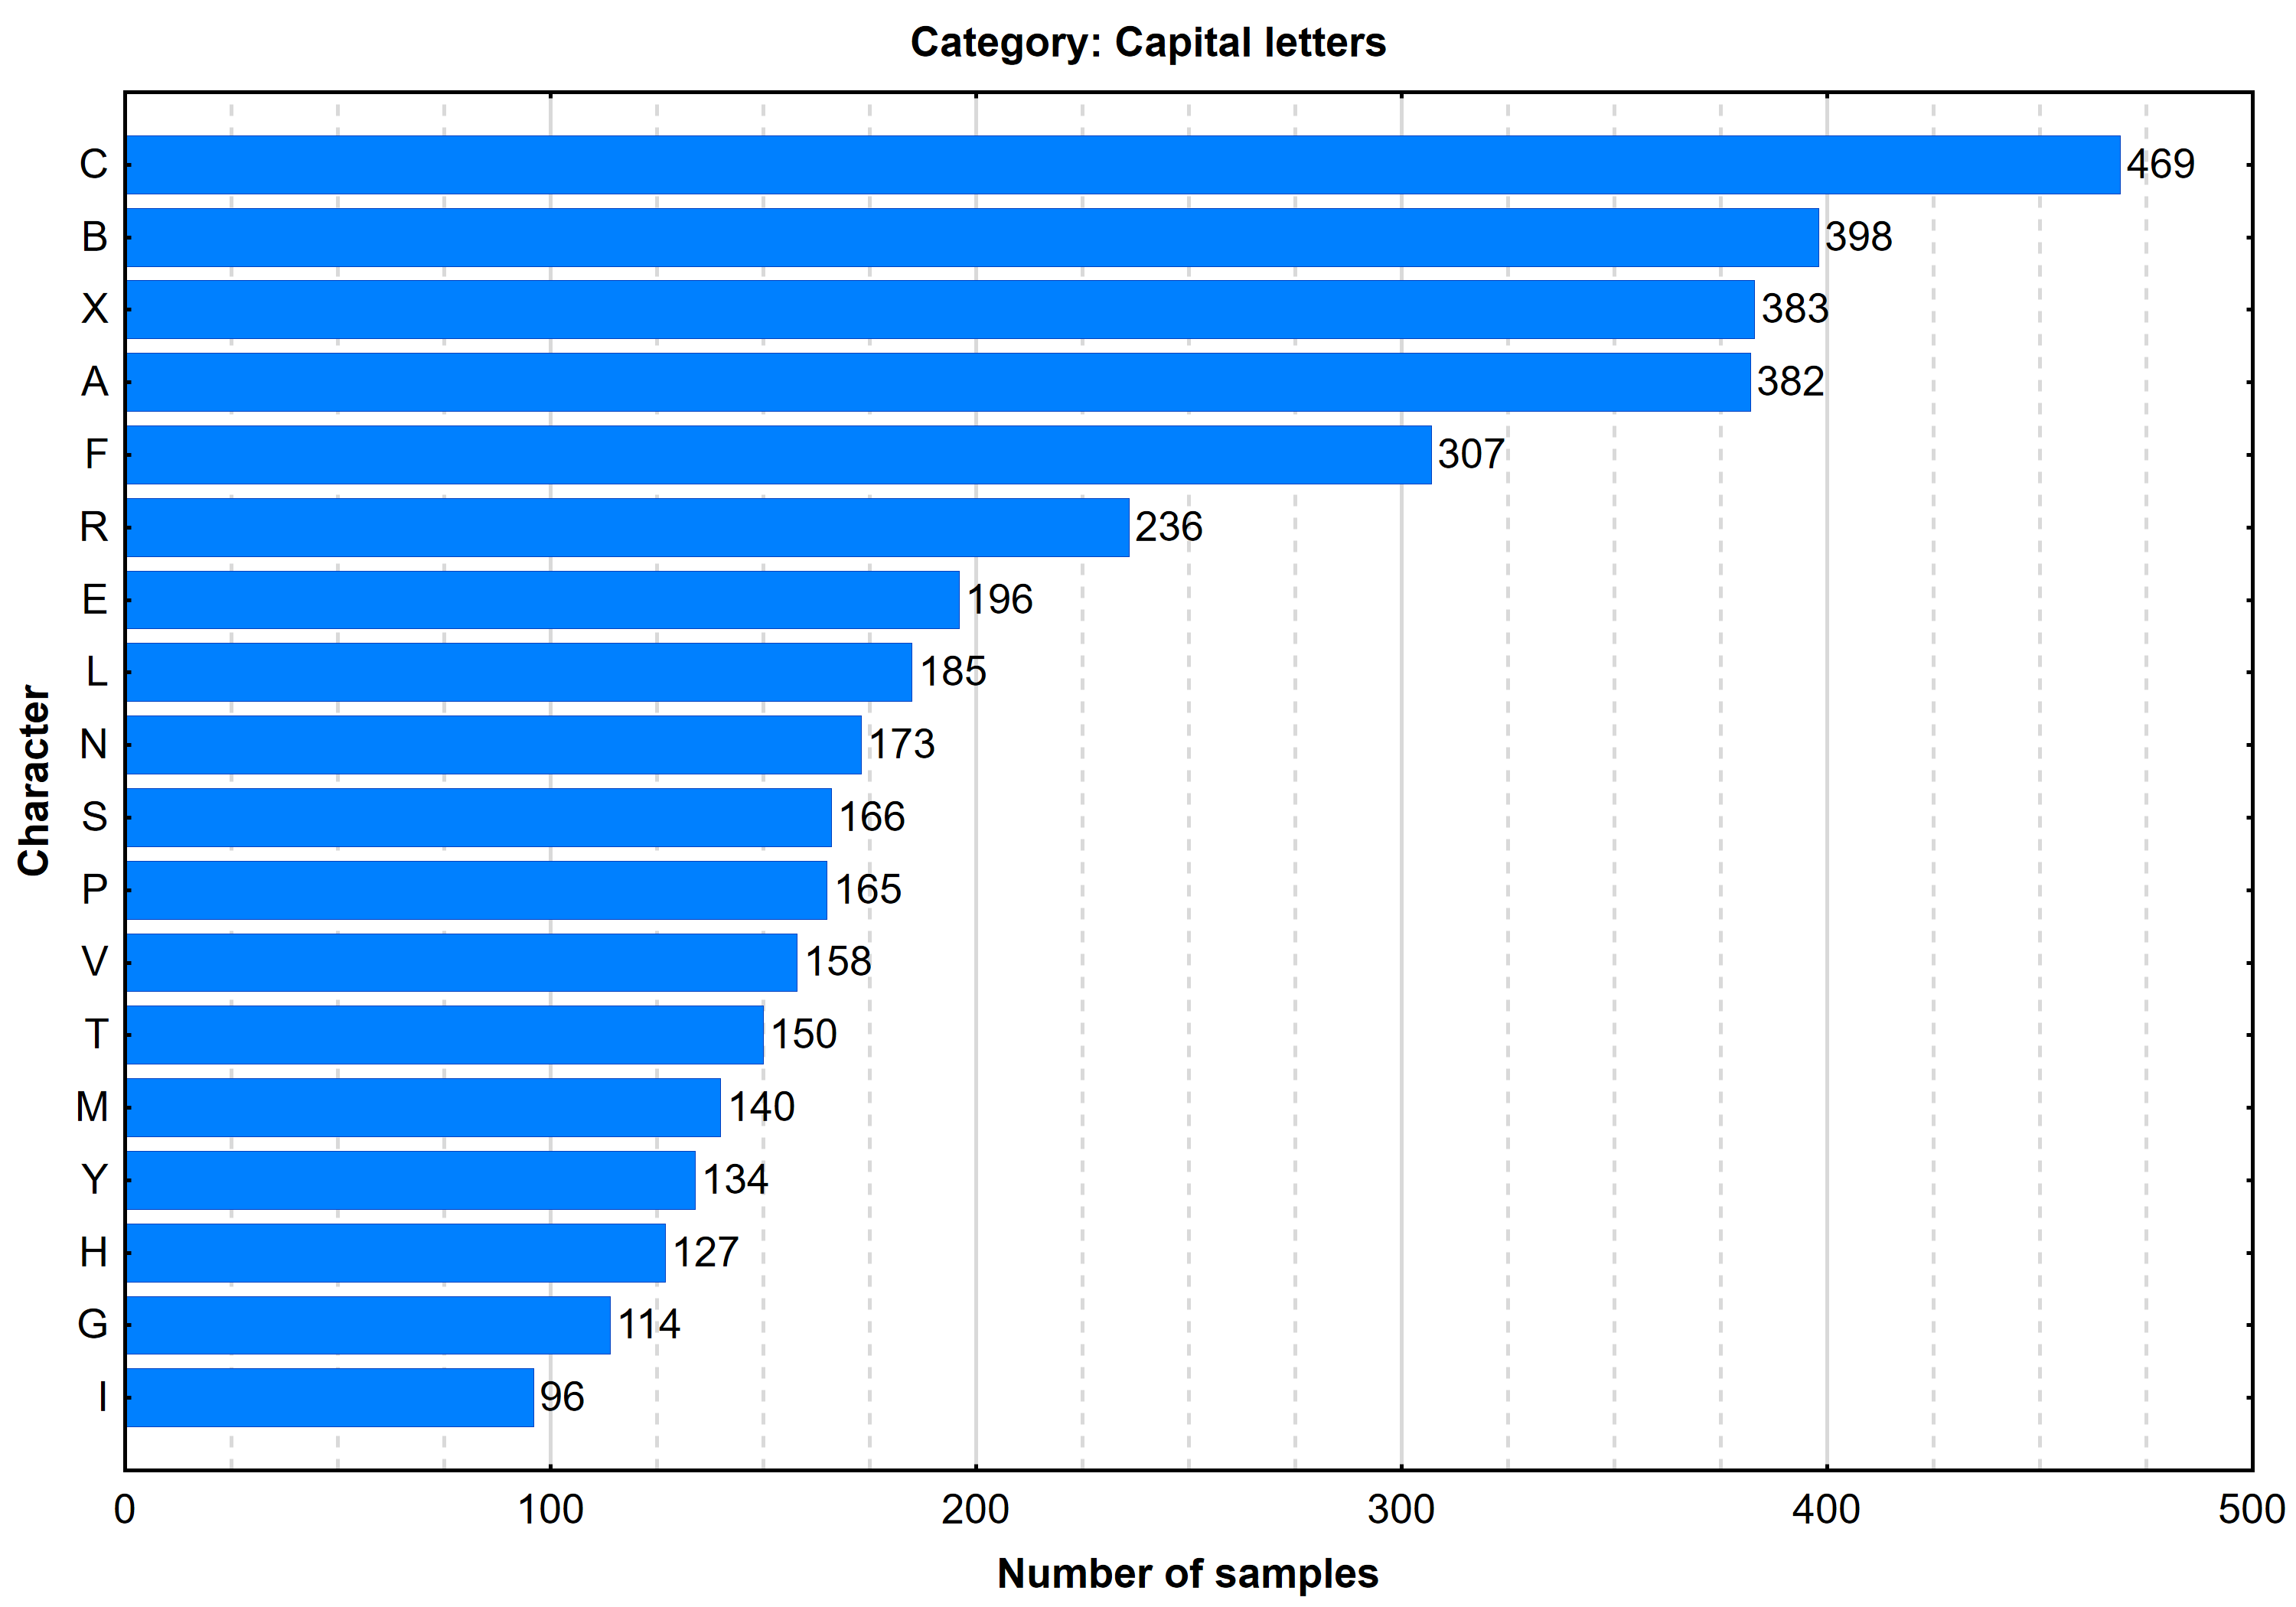
\includegraphics[width=1\textwidth]{capitulo3/imgs/capital_letters_distribution.png}
	\caption{Frecuencia de aparición de letras mayúsculas \cite{EXTRACTOR}}
	\label{fig:CapLetters}
\end{figure}
\newpage
En el caso de las letras minúsculas como podría esperarse la letra $\textbf{x}$ tiene la mayor aparición con ocho mil ciento nueve veces.
\begin{figure}[H]
	\centering
	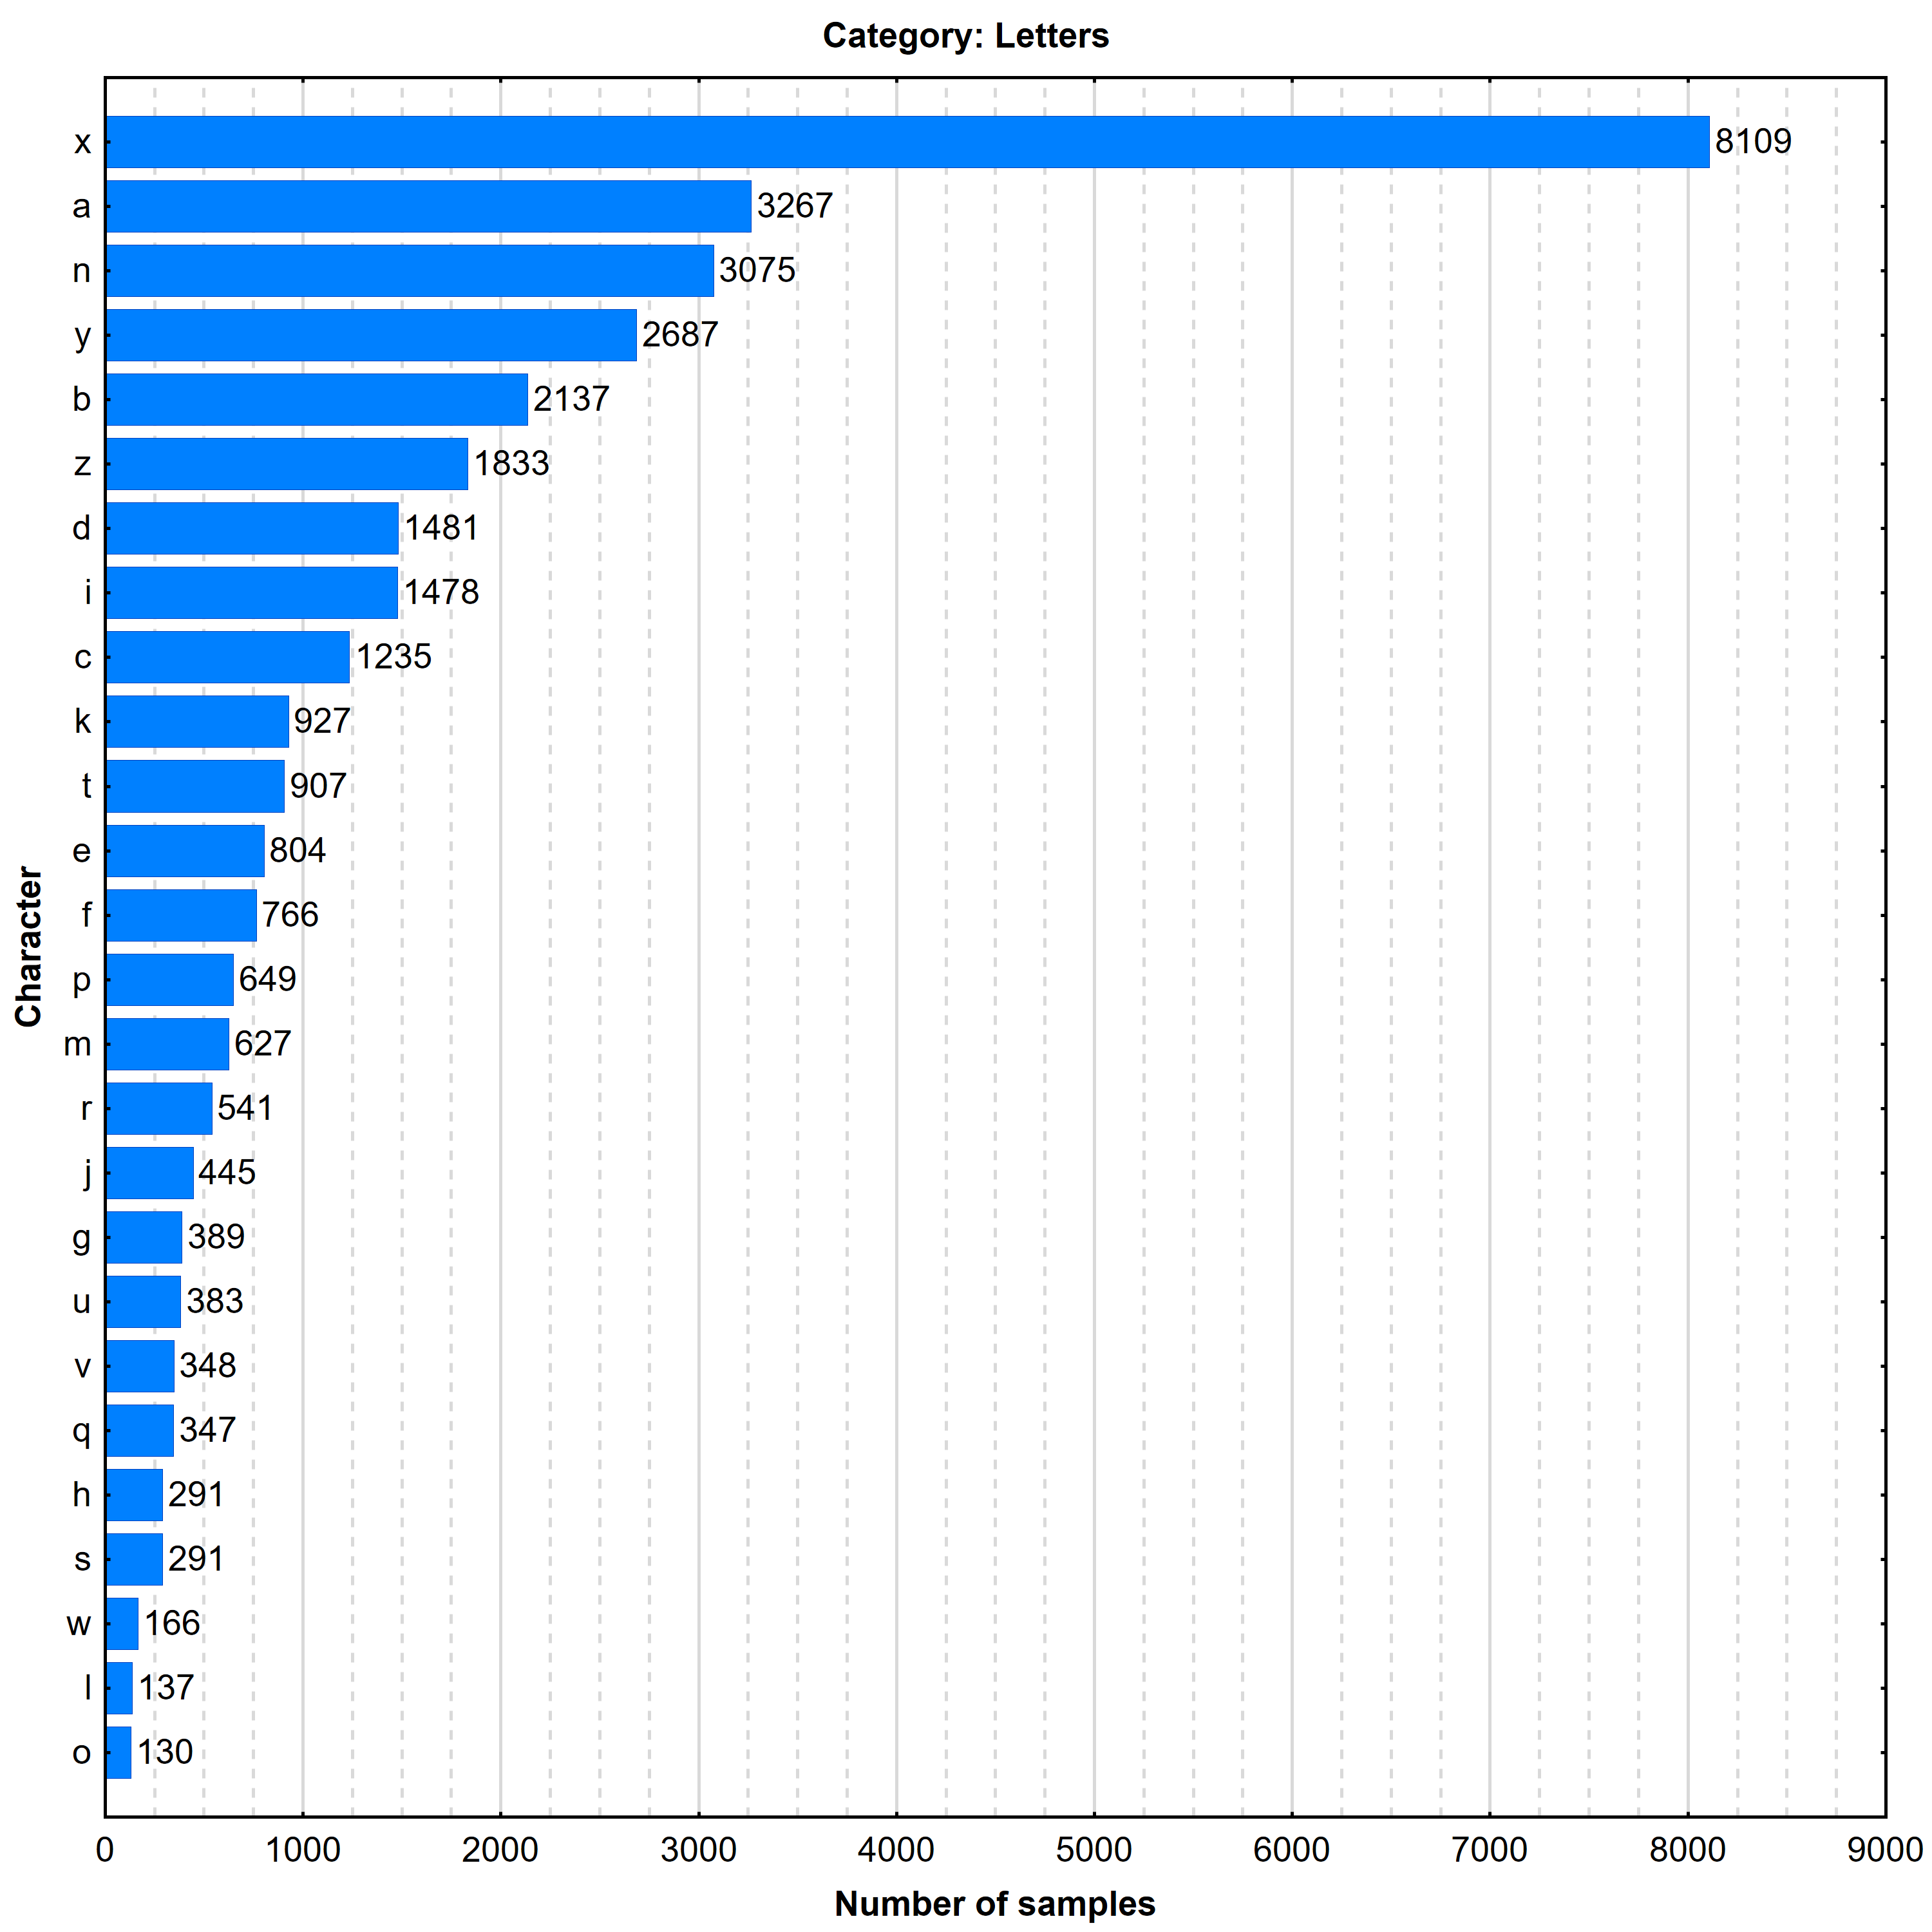
\includegraphics[width=1\textwidth]{capitulo3/imgs/lowercase_letters_distribution.png}
	\caption{Frecuencia de aparición de letras minúsculas \cite{EXTRACTOR}}
	\label{fig:LowerLetters}
\end{figure}
\newpage
La categoría con menos elementos pertenece a las letras griegas con nueve caracteres, siendo $\alpha$ (alpha) el de mayor aparición con ochocientas diecinueve veces.
\begin{figure}[H]
	\centering
	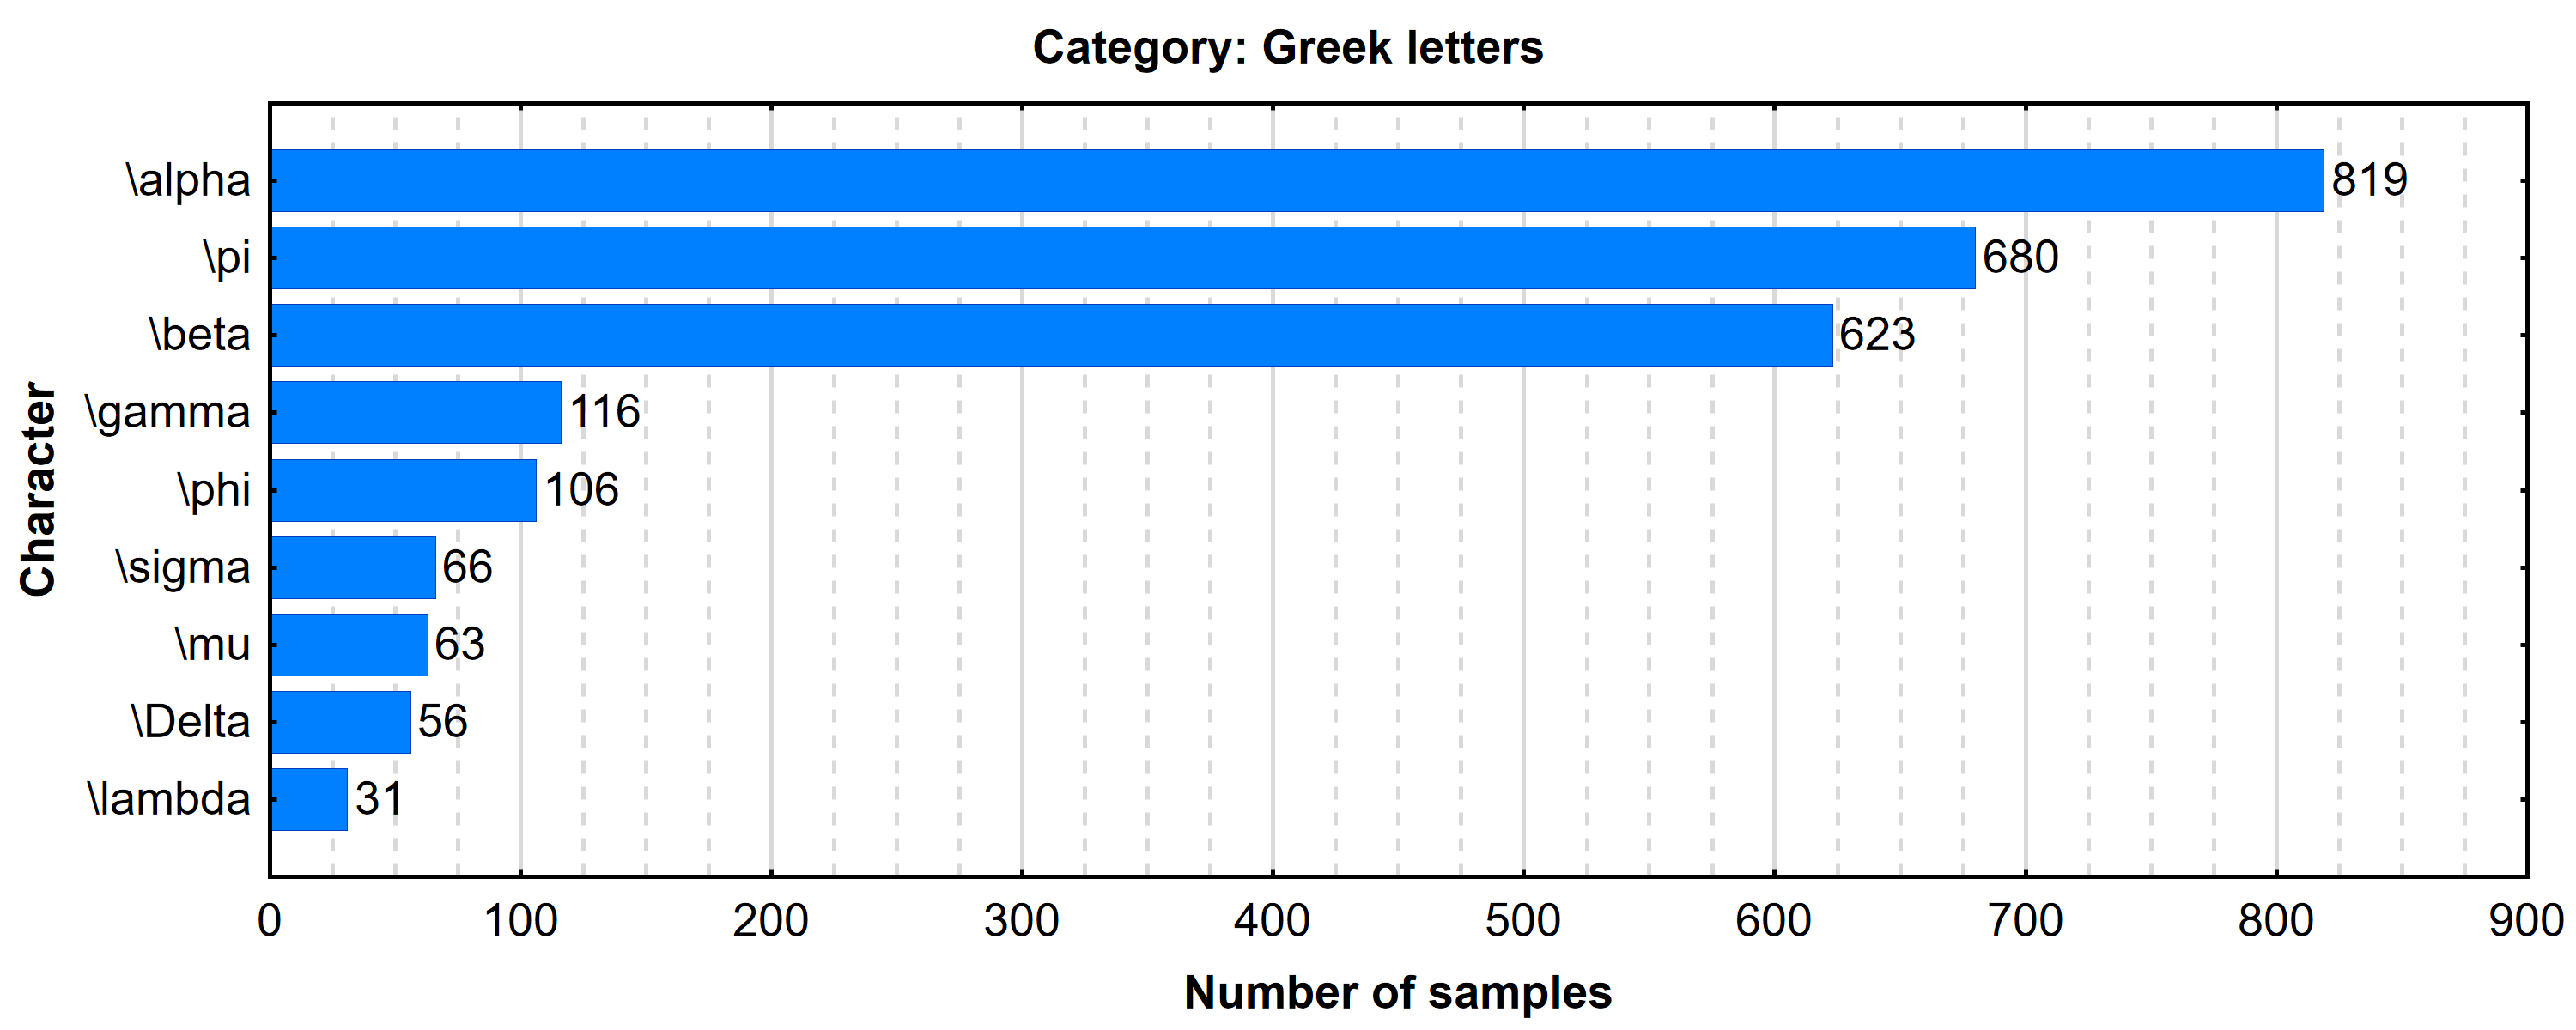
\includegraphics[width=1\textwidth]{capitulo3/imgs/greek_letters_distribution.png}
	\caption{Frecuencia de aparición de letras griegas \cite{EXTRACTOR}}
	\label{fig:GreekLetters}
\end{figure}
\newpage
Otros caracteres que aparecen en el conjunto de entrenamiento se muestran en la figura \ref{fig:SpecialSymbols} que son también de bastante utilidad como paréntesis, llaves, corchetes, el punto y la coma, que permiten definir jerarquía en las operaciones o números de punto flotante por mencionar dos aplicaciones que muestran la utilidad de los mismos. 
\begin{figure}[H]
	\centering
	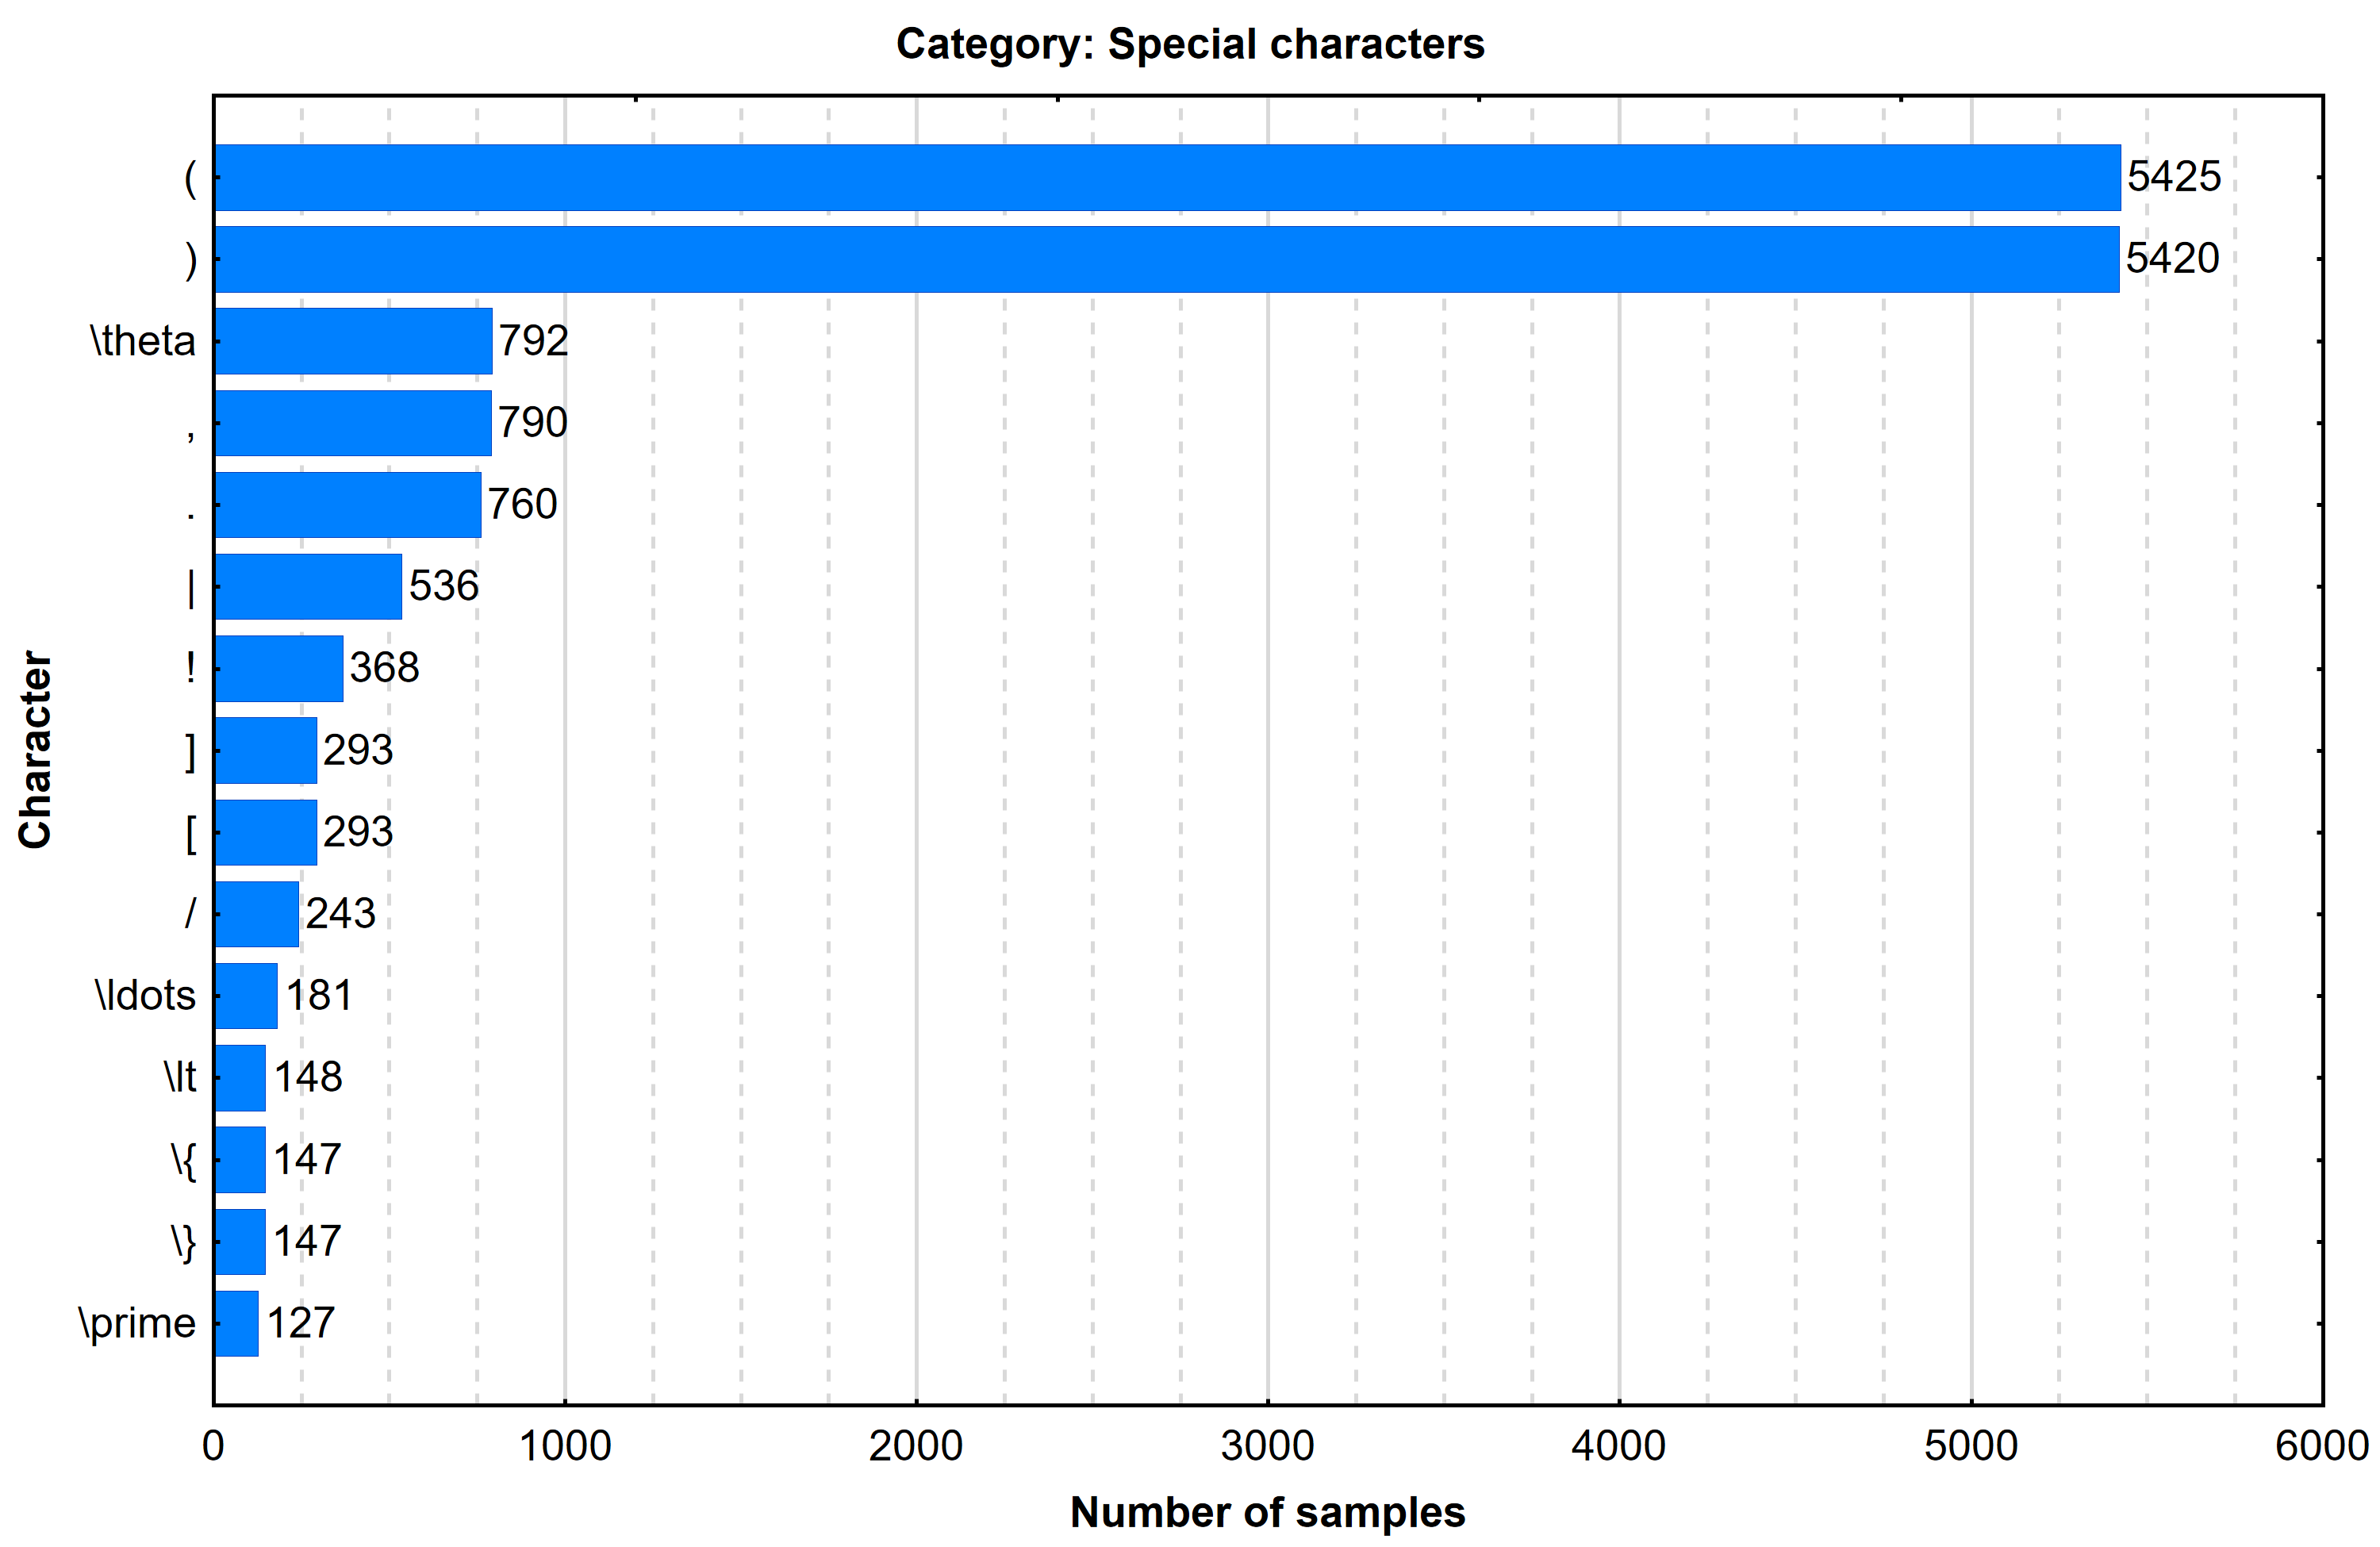
\includegraphics[width=1\textwidth]{capitulo3/imgs/special_characters_distribution.png}
	\caption{Frecuencia de aparición de símbolos especiales \cite{EXTRACTOR}}
	\label{fig:SpecialSymbols}
\end{figure}

Con estos histogramas se puede determinar qué símbolos se espera puedan ser reconocidos, así como aquellos de los cuales se esperan mejores resultados en función de su frecuencia de aparición en el conjunto de entrenamiento.

\newpage
\subsection{Nivel dimensional}
Sabiendo que el conjunto de entrenamiento CROHME no es lo suficientemente grande siendo esta una de las limitantes para obtener buenos resultados y teniendo en cuenta la bidimensionalidad que se presenta en las expresiones matemáticas, se propone el reconocimiento dos niveles en ambas direcciones, teniendo esta restricción con un mayor peso en dirección perpendicular al sentido de la escritura de las expresiones, esto basado en los resultados obtenidos por \cite{chino} 
con el mismo conjunto de entrenamiento. La figura \ref{fig:TwoDimensions} muestra un ejemplo del conjunto de entrenamiento CROHME.
%insertar Imagen
\begin{figure}[H]
	\centering
	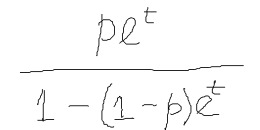
\includegraphics[width=0.6\textwidth]{capitulo3/imgs/twolevel.jpeg}
	\caption{Expresión de dos niveles vertical}
	\label{fig:TwoDimensions}
\end{figure}